\chapter{pH 与电导率滴定}\label{ch:g12:ph-conductivity-titrations}

一瓶葡萄酒醋的标签上写着“6 \% 酸度”，
即每 100 克醋中含 6 克乙酸。
乙酸及其共轭碱都没有颜色，高锰酸钾在这里也派不上用场。
但把 pH 计插入醋中，或者用一个测量导电能力的电导池，
随着逐滴加入的碱跟踪反应进程，曲线的形状准确显示出滴定终点的位置。
在实验台上花十分钟，
标签就可以核对了。

\begin{recall}
滴定、滴定终点与等当点体积
（\cref{ch:g11:titration}）；酸度常数（\cref{ch:g12:ka-and-pka}）；
亨德森关系式与指示剂
（\cref{ch:g12:buffers-predominance}）；离子溶液
能导电（\cref{ch:g9:ions}）。
\end{recall}

\begin{omfigure}
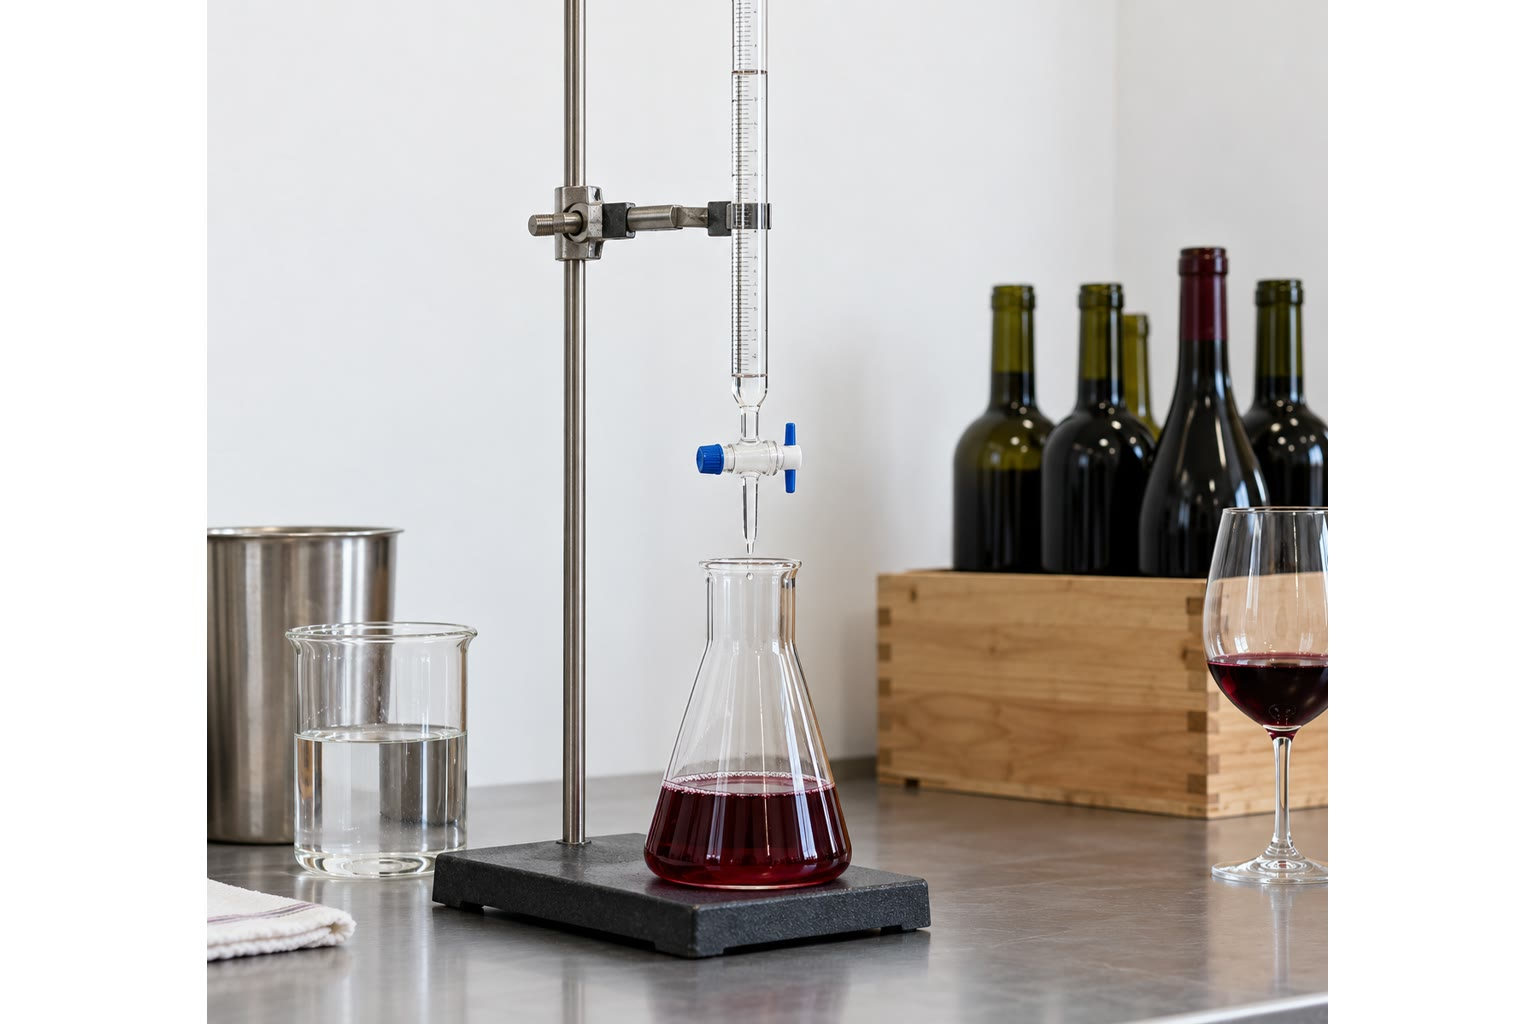
\includegraphics[width=0.45\linewidth]{images/book1/ai/g12-wine-lab.jpg}

{\small 酿酒师的滴定实验台。}
\end{omfigure}

\section{pH 滴定}

\begin{definition}[pH 滴定、半等当点]\label{def:g12:ph-conductivity-titrations:ph-metric}
在\emph{pH 滴定}\index{pH 滴定}中，被滴定溶液的
pH 在每次加入滴定剂后测定，并作出 pH 随所加体积变化的曲线。
\emph{半等当点}\index{半等当点}是指
已加入一半等当点体积时的那一点。
\end{definition}

\begin{omfigure}
\begin{tikzpicture}[font=\small, scale=0.65]
  \pic[transform shape] at (0,0) {stand={6.3}{2.0}};
  \pic[transform shape] at (2.0,0.68) {stirrer};
  \pic[transform shape] at (2.0,0.68) {beaker={0.45}{omWater}};
  \pic[transform shape] at (2.0,2.9) {burette={0.8}{omWater}};
  \pic[transform shape] (pr) at (2.6,0.95) {probe};
  \pic[transform shape] (m) at (6.4,3.4) {meter={pH}};
  \draw[black!70, thick] (pr-top) .. controls +(0,1.0) and +(0,-1.2) .. (m-a);
  \draw[omProp, thick, <-] (2.35,7.2) -- (4.3,7.6) node[right, text=black] {滴定管：NaOH};
  \draw[omProp, thick, <-] (1.4,1.1) -- (-1.4,1.6) node[left, text=black, align=right] {待滴定的酸};
  \draw[omProp, thick, <-] (2.75,2.4) -- (4.3,2.0) node[right, text=black] {pH 探头};
\end{tikzpicture}

{\small pH 滴定示意：探头浸入正在搅拌的溶液中，
pH 计显示每次加入后的 pH。}
\end{omfigure}

\begin{inthelab}[校准 pH 计]
使用前，先用蒸馏水冲洗探头，再将其浸入两种
pH 已知的缓冲溶液中（通常为 7.0 和 4.0，或 10.0），并将 pH 计
调至显示这些溶液的标准值。两种溶液之间，探头需冲洗并
轻轻吸干，切勿擦拭；保存时探头尖端保持湿润。
\end{inthelab}

\begin{omfigure}
\begin{minipage}{0.49\linewidth}
\begin{tikzpicture}
\begin{axis}[width=\linewidth, height=6cm, xmin=0, xmax=30, ymin=0, ymax=14,
    xlabel={$V_{\text{NaOH}}$ (\si{mL})}, ylabel={pH}, axis lines*=left,
    ymajorgrids, grid style={gray!20}, tick label style={font=\scriptsize},
    label style={font=\small}, title={\small \ce{HCl}（用 \ce{NaOH} 滴定）},
    title style={yshift=-4pt}]
  \addplot[very thick, omDef] table[x=V, y=pH] {figdata/out/grade-12-ph-conductivity-titrations-a.dat};
  \addplot[thick, omProp, densely dotted] table[x=V, y expr=\thisrow{dpH}/4]
    {figdata/out/grade-12-ph-conductivity-titrations-a.dat};
  \addplot[dashed, black!60] coordinates {(20,0) (20,7)};
  \node[font=\scriptsize, anchor=north west] at (axis cs:20.3,6.5) {$V_E = 20.0$};
\end{axis}
\end{tikzpicture}
\end{minipage}\hfill
\begin{minipage}{0.49\linewidth}
\begin{tikzpicture}
\begin{axis}[width=\linewidth, height=6cm, xmin=0, xmax=16, ymin=0, ymax=14,
    xlabel={$V_{\text{NaOH}}$ (\si{mL})}, ylabel={pH}, axis lines*=left,
    ymajorgrids, grid style={gray!20}, tick label style={font=\scriptsize},
    label style={font=\small}, title={\small \ce{CH3COOH}（用 \ce{NaOH} 滴定）},
    title style={yshift=-4pt}]
  \addplot[very thick, omDef] table[x=V, y=pH] {figdata/out/grade-12-ph-conductivity-titrations-b.dat};
  \addplot[thick, omProp, densely dotted] table[x=V, y expr=\thisrow{dpH}/4]
    {figdata/out/grade-12-ph-conductivity-titrations-b.dat};
  \addplot[dashed, black!60] coordinates {(10.1,0) (10.1,8.7)};
  \addplot[dashed, black!60] coordinates {(0,4.76) (5.05,4.76) (5.05,0)};
  \node[font=\scriptsize, anchor=south west] at (axis cs:0.2,4.8) {$pK_a = 4.76$};
  \node[font=\scriptsize, anchor=north west] at (axis cs:10.4,3.0) {$V_E = 10.1$};
\end{axis}
\end{tikzpicture}
\end{minipage}

{\small 计算得到的 pH 曲线（蓝色）及其导数 $d\mathrm{pH}/dV$
（橙色，点线，已除以 4）。左图：\qty{20.0}{mL} 盐酸，
浓度为 \qty{0.100}{mol/L}；滴定终点位于 pH 7.00。右图：\qty{10.0}{mL}
稀释醋；在半等当点处 pH 等于 $pK_a$，而
滴定终点位于碱性 pH 处。}
\end{omfigure}


\begin{method}[导数法]\label{met:g12:ph-conductivity-titrations:derivative}
在相邻两次测量之间计算斜率
$\Delta\mathrm{pH}/\Delta V$，并对 $V$ 作图（可用电子表格或
计算器完成）。等当点体积即斜率最大处，
也就是导数曲线的峰值。
\end{method}

\begin{method}[切线法]\label{met:g12:ph-conductivity-titrations:tangent}
\begin{enumerate}
  \item 在曲线上作两条平行切线，一条位于跃变之前，
        一条位于跃变之后，分居跃变两侧。
  \item 作出位于两切线中间的平行线。
  \item 该平行线与曲线的交点即为滴定终点，读出 $V_E$（及
        滴定终点处的 pH）。
\end{enumerate}
\end{method}

\begin{proposition}[半等当点处，$\mathrm{pH} = pK_a$]\label{prop:g12:ph-conductivity-titrations:half}
在用强碱滴定弱酸 \ce{HA} 的过程中，
半等当点处 $\mathrm{pH} = pK_a$。
\end{proposition}

\begin{proof}
反应 \ce{HA + OH- -> A- + H2O} 进行得很彻底。在半等当点处，一半
的酸已转化为 \ce{A-}，即 $[\ce{A-}] = [\ce{HA}]$，
由亨德森关系式可得 $\mathrm{pH} = pK_a + \log 1 = pK_a$。
\end{proof}

\begin{remark}[从曲线选择指示剂]\label{rem:g12:ph-conductivity-titrations:indicator}
% ledger: ind:BBT, ind:phenolphthalein
指示剂必须在跃变范围内变色。对于盐酸，
跃变范围约为 pH 4 至 10，许多指示剂都适用，其中溴百里酚蓝
效果最好；对于乙酸，跃变范围较窄且偏碱性，约为 7 至 11：
酚酞（8.0--10.0）适用，溴百里酚蓝
则会过早变色。
\end{remark}

\section{电导率与电导滴定}

\begin{definition}[电导率，离子摩尔电导率]\label{def:g12:ph-conductivity-titrations:conductivity}
溶液的\emph{电导率}\index{电导率} $\sigma$ 表示其导电能力的强弱，
其值用电导率仪读取，
单位为 \si{mS/cm}（或 \si{S/m}）。每种离子 $i$ 对电导率的贡献
与其浓度成正比，比例系数为 $\lambda_i$，
即其\emph{离子摩尔电导率}\index{离子摩尔电导率}。
\end{definition}

\begin{proposition}[科尔劳施定律]\label{prop:g12:ph-conductivity-titrations:kohlrausch}
% ledger: lam:H+, lam:OH-, lam:Na+, lam:Cl-
对于稀溶液，$\sigma = \sum_i \lambda_i [X_i]$。
在 \qty{25}{\celsius} 下（单位为 \si{S.cm^2/mol}）：\ce{H3O+} 349.8、\ce{OH-} 198.3、
\ce{Cl-} 76.2、\ce{Na+} 50.3。水合氢离子和氢氧根离子的导电能力
远强于其他所有离子。
\end{proposition}

\begin{proof}
在本阶段不加证明地承认（证明见本科一年级分册）。\ce{Cl-} 与 \ce{Na+} 的数值来自
盐酸和氯化钠溶液的实测电导率，
由此扣去其他离子的贡献，即得 \ce{H3O+} 的数值。
\end{proof}

\begin{definition}[电导滴定]\label{def:g12:ph-conductivity-titrations:conductimetric}
在\emph{电导滴定}\index{电导滴定}中，每加入一次滴定剂后
测定一次电导率。被滴定溶液
稀释于大量水中，使所加体积
几乎不改变其浓度，因此各数据点落在直线上，
这些直线在滴定终点处斜率发生改变。
\end{definition}

\begin{omfigure}
\begin{minipage}{0.4\linewidth}\centering
\begin{tikzpicture}[font=\small, scale=0.75]
  \pic[transform shape] at (0,0) {beaker={0.6}{omWater}};
  \pic[transform shape] (cc) at (0.2,0.2) {condcell};
  \pic[transform shape] (m) at (2.6,3.4) {meter={mS/cm}};
  \draw[black!70, thick] (cc-top) .. controls +(0,0.8) and +(0,-1) .. (m-a);
  \node[anchor=north, align=center] at (0.6,-0.15) {电导池 \\ 位于溶液中};
\end{tikzpicture}
\end{minipage}\hfill
\begin{minipage}{0.56\linewidth}
\begin{tikzpicture}
\begin{axis}[width=\linewidth, height=5.4cm, xmin=0, xmax=20, ymin=0,
    ymax=4.6, xlabel={$V_{\text{NaOH}}$ (\si{mL})}, ylabel={$\sigma$ (\si{mS/cm})},
    axis lines*=left, ymajorgrids, grid style={gray!20},
    tick label style={font=\scriptsize}, label style={font=\small}]
  \addplot[only marks, mark=*, mark size=1.4pt, omDef] table[x=V, y=sigma]
    {figdata/out/grade-12-ph-conductivity-titrations-c.dat};
  \addplot[dashed, black!60] coordinates {(10,0) (10,4.6)};
  \node[font=\scriptsize, anchor=south west] at (axis cs:10.3,0.2) {$V_E = 10.0$};
\end{axis}
\end{tikzpicture}
\end{minipage}

{\small 左：电导池。右：\qty{100}{mL} 盐酸，
浓度为 \qty{0.0100}{mol/L}，用氢氧化钠溶液滴定，其浓度为
\qty{0.100}{mol/L}（按科尔劳施定律计算）。电导率先
下降后上升：两条直线在滴定终点处相交。}
\end{omfigure}

\begin{example}[读取两条直线]\label{ex:g12:ph-conductivity-titrations:lines}
滴定终点之前，每加入一个 \ce{OH-}，便消耗一个 \ce{H3O+}
（$\lambda = 349.8$），并引入一个 \ce{Na+}（$\lambda = 50.3$），
电导率急剧下降。滴定终点之后，\ce{Na+} 与 \ce{OH-}
（$\lambda = 198.3$）只是不断积累，电导率随之上升。两条直线
相交于 $V_E = \qty{10.0}{mL}$，因此酸的浓度为
$0.100 \times 10.0 / 100 = \qty{0.0100}{mol/L}$。
\end{example}

\begin{method}[由电导滴定确定滴定终点]\label{met:g12:ph-conductivity-titrations:two-lines}
先对滴定终点之前的数据点，及终点之后的数据点，分别作最佳拟合直线，
再读取两直线交点处的 $V_E$。
靠近滴定终点、直线发生弯曲的数据点
应舍去。
\end{method}

\begin{remark}[何时选用何种方法]\label{rem:g12:ph-conductivity-titrations:which}
若有合适的有色指示剂，则最为快捷。pH 滴定
也可求出弱酸的 $pK_a$，且适用于有色或浑浊的溶液。
电导滴定则完全不需要 pH 跃变：
它适用于极弱或极稀的酸，也适用于沉淀反应，
只要离子发生变化即可。
\end{remark}

\begin{safety}{\ghs[0.82cm]{GHS05}\ghs[0.82cm]{GHS07}}
% ledger: ghs:NaOH
氢氧化钠溶液会灼伤皮肤和眼睛，即便是稀溶液
  也会灼伤眼睛：全程佩戴护目镜，任何溅出的液体
都应立即用大量水冲洗。
\end{safety}

\section{练习}


\begin{exercise}[$\star$]\label{exo:g12:ph-conductivity-titrations:1}
读出盐酸被氢氧化钠滴定时曲线上的等当点体积，
所用氢氧化钠浓度为 \qty{0.100}{mol/L}，
并求出 \qty{20.0}{mL} 盐酸的浓度。
\end{exercise}

\begin{exercise}[$\star$]\label{exo:g12:ph-conductivity-titrations:2}
用氢氧化钠滴定一弱酸；$V_E = \qty{12.0}{mL}$。在
\qty{6.0}{mL} 时 pH 为 3.75。求该酸的 $pK_a$，
并指出它可能是 $pK_a$ 标度上的哪一种酸？
\end{exercise}

\begin{exercise}[$\star$]\label{exo:g12:ph-conductivity-titrations:3}
用氢氧化钠滴定乙酸时，应选用哪种指示剂？
为什么不用甲基红？
\end{exercise}

\begin{exercise}[$\star$]\label{exo:g12:ph-conductivity-titrations:4}
为什么使用 pH 计前必须校准？用什么来校准？
\end{exercise}

\begin{exercise}[$\star$]\label{exo:g12:ph-conductivity-titrations:5}
利用离子摩尔电导率，将 \ce{H3O+}、\ce{OH-}、
\ce{Na+}、\ce{Cl-} 按导电能力从强到弱排序。
\end{exercise}

\begin{exercise}[$\star\star$]\label{exo:g12:ph-conductivity-titrations:6}
\qty{20.0}{mL} 乙酸溶液恰好用去 \qty{14.6}{mL}
浓度为 \qty{0.050}{mol/L} 的氢氧化钠溶液。求该乙酸溶液的浓度。
\end{exercise}

\begin{exercise}[$\star\star$]\label{exo:g12:ph-conductivity-titrations:7}
在等当点附近，读数如下：\qty{9.6}{mL}，pH 5.7；
\qty{9.8}{mL}，6.1；\qty{10.0}{mL}，7.0；\qty{10.2}{mL}，10.5；
\qty{10.4}{mL}，11.0。计算相邻两点之间的
$\Delta\mathrm{pH}/\Delta V$，并定出 $V_E$。
\end{exercise}

\begin{exercise}[$\star\star$]\label{exo:g12:ph-conductivity-titrations:8}
在盐酸的电导滴定中，结合溶液中存在的离子，
解释等当点前后斜率的符号。
\end{exercise}

\begin{exercise}[$\star\star$]\label{exo:g12:ph-conductivity-titrations:9}
画出以氢氧化钠滴定乙酸的电导滴定曲线示意图，
并解释为什么在等当点之前电导率就已上升？
\end{exercise}

\begin{exercise}[$\star\star$]\label{exo:g12:ph-conductivity-titrations:10}
在稀释后醋的计算曲线上，读出开始时的 pH、
半等当点与等当点处的 pH。为什么起始 pH 远高于
同浓度盐酸的起始 pH？
\end{exercise}

\begin{exercise}[$\star\star$]\label{exo:g12:ph-conductivity-titrations:11}
为什么在电导滴定前要把被滴定溶液
用大量水稀释？
\end{exercise}

\begin{exercise}[$\star\star\star$]\label{exo:g12:ph-conductivity-titrations:12}
某溶液同时含有盐酸和乙酸。
用氢氧化钠滴定该溶液并测量 pH，解释
为什么曲线出现两次跃变，以及每个等当点体积各测量的是什么。
\end{exercise}

\begin{exercise}[$\star\star\star$]\label{exo:g12:ph-conductivity-titrations:13}
计算本章电导滴定开始时的电导率，
（\qty{0.0100}{mol/L} 盐酸）与等当点时的
（\qty{110}{mL} 氯化钠溶液）的电导率，并与图对比。
\end{exercise}

\begin{exercise}[$\star\star\star$]\label{exo:g12:ph-conductivity-titrations:14}
一台校准很差的 pH 计，每次读出的 pH 都偏高 0.2。它对 pH 滴定的
等当点体积造成什么误差？对
半等当点处读出的 $pK_a$ 有什么影响？
\end{exercise}

\begin{exercise}[$\star\star\star$]\label{exo:g12:ph-conductivity-titrations:15}
为什么电导滴定能够跟踪银离子与氯离子的反应，
\ce{Ag+ + Cl- -> AgCl(s)}，而 pH 滴定则不能？
描述向氯化钠溶液中加入硝酸银时预期的曲线
（取 \ce{NO3-} 的 $\lambda$ 与
\ce{Cl-} 的相近）。
\end{exercise}

\section{问题：醋的酸度是否为 6\,\%？}

\begin{problem}[{周末问题——标称“6 \%
酸度”的醋，真的每百克含六克乙酸吗？}]
\label{pb:g12:ph-conductivity-titrations:1}
% ledger: pka:ethanoic, ind:phenolphthalein, lam:OH-, lam:Na+, aw:C, aw:H, aw:O
对一瓶标示“6 \%酸度”的醋进行检验。取其 \qty{100.0}{mL}
称得质量为 \qty{101}{g}。将醋稀释十倍，然后
取稀释后的溶液 \qty{10.0}{mL}，用氢氧化钠滴定，
所用氢氧化钠浓度为 \qty{0.100}{mol/L}，用 pH 计测量；本章的计算曲线
（右图）与测量结果吻合。

\medskip
\noindent\textbf{第一部分——样品的准备。}
\begin{enumerate}
  \item “6 \%酸度”是什么意思？
  \item 若标签正确，\qty{100.0}{mL} 醋中
        应含乙酸多少质量？其物质的量
        浓度是多少？
  \item 为什么滴定前要将醋稀释？
  \item 稀释为原来的十倍应使用哪种玻璃仪器？
\end{enumerate}

\medskip
\noindent\textbf{第二部分——pH 滴定。}
\begin{enumerate}[resume]
  \item 写出滴定反应的方程式。
  \item 在曲线上读出等当点体积。
  \item 计算稀释后醋的浓度。
  \item 由此推出醋的浓度。
  \item 读出半等当点处的 pH。它说明了什么？
  \item 为什么等当点处的 pH 大于 7？
  \item 哪种指示剂可得到相同的结果？
\end{enumerate}

\medskip
\noindent\textbf{第三部分——电导滴定核对。}
\begin{enumerate}[resume]
  \item 用电导池重复滴定，样品
        稀释于 \qty{200}{mL} 水中。等当点之前，
        溶液中出现哪些离子？
  \item 为什么等当点之前电导率只缓慢上升？
  \item 为什么等当点之后上升得更快？
  \item 为什么开始时电导率很低？
  \item 两条直线应在何处相交？
\end{enumerate}

\medskip
\noindent\textbf{第四部分——结论。}
\begin{enumerate}[resume]
  \item 计算醋中乙酸的质量浓度。
  \item 计算 \qty{100.0}{mL} 醋中乙酸的质量。
  \item 推出每 \qty{100}{g} 醋中乙酸的质量。
  \item 给出最终结论：这份醋的酸度是多少？
\end{enumerate}
\end{problem}
